\chapter{Results}%
\label{ch:results}

Due to the lack of existing solutions, an evaluation framework was programmed to evaluate the performance of our proposed algorithm. The framework consists of different models presented in the literature, the majority of which had been implemented in the pyGAM \cite{serven2018pygam} library but integrated into our toolkit with support for hyperparameter optimisation and cross-validation using scikit-learn \cite{scikit-learn}. We hope this creates a unified framework for future developments to make the evaluation process transparent and reproducible.


As discussed in sections \ref{sec:tristimulus} and \ref{ss:colour}, the responses for both the camera and the standard observer can be synthesised knowing the spectral sensitivities, illuminant SPD and surface reflectances. For training and evaluation, we simulate the responses of the cameras and the observer by using a known set of spectral sensitivities. This allows us to generate synthetic responses for available reflectance and illumination spectrum combinations. In the subsequent chapters, we will explain acquiring the required spectral information.

\section{Reflectance dataset}
\label{sec:data}
Since the camera spectral sensitivities are typically not a linear combination of the XYZ colour-matching functions, a perfect transform that would map each surface correctly to its XYZ counterpart cannot be found with linear methods. Some might get mapped correctly under one illuminant, thus making them a metameric match, a phenomenon discussed in \ref{ss:metamerism}. This can not be avoided, but by selecting a proper dataset, we can adjust our transformation to be more correct for certain surfaces, such as human skin. For example, in the case of a smartphone front camera characterisation, it would be more beneficial to map skin tones correctly rather than the environment since the front camera is often used for selfies \cite{imatest2024skin}. 

Thanks to the rise of hyperspectral imaging, various publications exist regarding the spectral reflectances of scenes. While many of them do not directly discuss the problem of colour correction, they often include per-pixel data of nature and city landscapes, vegetation, and human-made objects, making them an excellent tool for correcting the colours of typical objects that might be photographed. The most common target for colour correction is the 24-patch ColorChecker calibration chart \cite{mccamy1976color}, for which spectral reflectances are widely available. The different patches are shown in Figure \ref{fig:macbeth}, and their chromaticities are demonstrated along the border of the sRGB gamut in Figure \ref{fig:macbeth_chromaticity}. Although the chart contains some colours typically seen in nature, such as skin tones and vegetation, those are few and do not sufficiently represent the scenes we regularly photograph \cite{wueller2009situ}. Variations with more patches exist, such as the ColorChecker Digital SG \cite{calibrite}, but those exhibit the same problem. 

In the absence of the camera's spectral sensitivities under calibration, these colour charts provide a fast and cheap way for camera colour calibration. One can take a RAW image of the chart under a known illuminant and compute (or measure using a spectrophotometer) the corresponding target XYZ values. A simple 3x3 matrix is then found through regression, as is done when the spectral sensitivities are known.

\begin{figure}
    \centering
    \pdftooltip{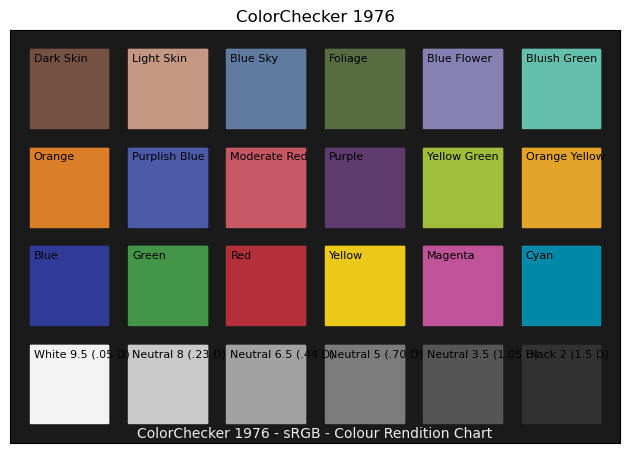
\includegraphics[width=\textwidth]{figures/macbeth.png}}{macbeth}
    \caption{Macbeth ColorChecker from 1976 \cite{mccamy1976color}.}
    \label{fig:macbeth}
\end{figure}

\begin{figure}
    \centering
    \pdftooltip{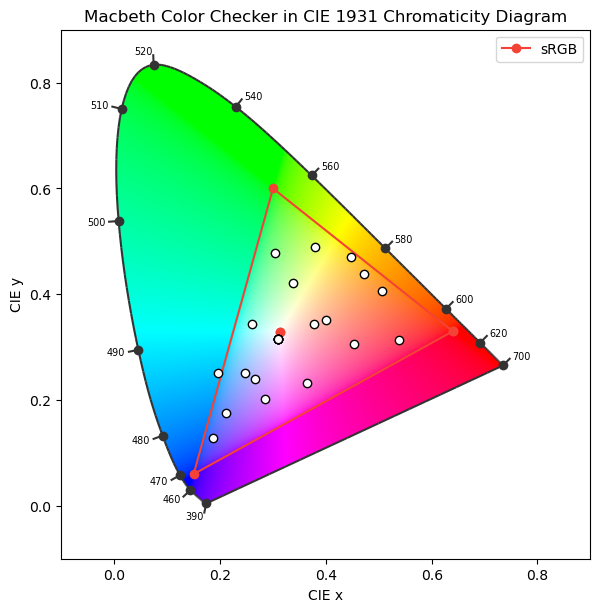
\includegraphics[scale=0.8]{figures/macbeth_chromaticity.png}}{MCC}
    \caption{Macbeth ColorChecker patches visualised along the sRGB gamut in the CIE 1931 Chromaticity Diagram.}
    \label{fig:macbeth_chromaticity}
\end{figure}


Another problem frequently seen with colour checkers is that they are used as training and testing data. If we measure the error on the training set we used, it will be small as it can be overfitted to the training data. Furthermore, the low error gives us no guarantee the algorithm will perform well outside this limited dataset. For practical results, it would thus be ideal to have training and test datasets that are different but representative of the actual distribution of colours in the real world. To alleviate this problem, we collected three datasets published in the literature with more natural distribution: nature and city landscapes, vegetation, and human-made objects.

The multispectral dataset published by Columbia Imaging and Vision Laboratory (CAVE) \cite{CAVE_0293} has been widely used in publications on hyperspectral imaging. Figure \ref{fig:cave} shows some of the imaged objects, from which it is apparent that the dataset consists of a wide variety of objects, even artificial ones. 

\begin{figure}
    \centering
    \pdftooltip{\includegraphics[width=\textwidth]{figures/cave.png}}{cave}
    \caption{Objects tested under the CAVE multispectral dataset \cite{CAVE_0293}.}
    \label{fig:cave}
\end{figure}

\begin{figure}
    \centering
    \pdftooltip{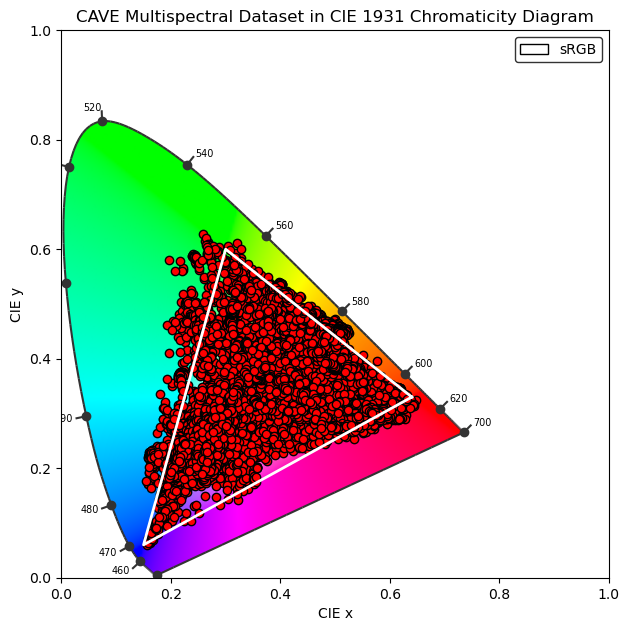
\includegraphics[scale=0.8]{figures/cave_gamut.png}}{cave}
    \caption{Cave multispectral dataset (after dimensionality reduction) visualised along the sRGB gamut in the CIE 1931 Chromaticity Diagram.}
    \label{fig:cave_gamut}
\end{figure}

The published dataset was released as a set of images, each representing a single band of a captured hyperspectral image. Thirty-one bands were collected per image, from 400 to 700 nm at 10 nm intervals. Since there are 32 images of size 512$\times$512, the number of distinct reflectances is roughly 8.8 million. In theory, this amount of training data could help train complex algorithms. However, looking at any singular pixel, it can be observed that the ones near it are very similar and do not add significant new information to the training process. Thus, the images were resized to the size of 32$\times$32. In Figure \ref{fig:cave_gamut}, we see the chromaticity gamut of the dataset after resizing. It is apparent that even after the dimensionality was significantly reduced, it still occupies a large area of the sRGB gamut, even containing many samples outside it.

Although the CAVE multispectral dataset consists of everyday objects encountered, it lacks colours encountered in natural scenes, such as urban environments and vegetation, which typically occupy the majority of photographed images. For evaluating the performance of colour constancy algorithms, \citeauthor{Foster:06} has released three datasets \cite{Foster:06},\cite{Foster2022}, \cite{foster:2002} of natural scenes in Minho region, Portugal. Figure \ref{fig:foster} showcases the scenes photographed in \cite{Foster2022}. The dataset clearly captures various natural colours, from urban environments to vegetation, such as leaves and flowers. In Figure \ref{fig:foster50gamut}, we also see the chromaticity gamut of the dataset "Foster 50 Reduced Hyperspectral Reflectance
Images", which reveals that it occupies an even more extensive area of the visible gamut than the CAVE multispectral dataset.

Since some of the images in \cite{Foster:06} and \cite{Foster2022} were found to be identical, we only consider the datasets in \cite{foster:2002} and \cite{Foster2022} from \citeauthor{Foster2022}. In order to create a diverse dataset for training, we combine the data from \cite{CAVE_0293} and \cite{foster:2002} into one larger dataset with 39935 samples, denoted as "CAVE/Foster020202"  in the subsequent analysis. As an alternative dataset, to see how the training set size affects the models, we use the InSitu dataset with a total of 1961 samples. We save the dataset from \cite{Foster2022}, denoted as Foster50, entirely for testing as it was found too large to train some of the algorithms with 204800 samples. One might argue, that using the Foster02 in the training dataset while evaluating on the Foster50, which contains similar scenes, would lead to the models learning the distribution of the testing set. However, the Foster02 dataset contains relatively few samples compared to the CAVE dataset also used in training; with both also being significantly different, the slight similarity in train and testing samples is not considered an issue.


\begin{figure}
    \centering
    \pdftooltip{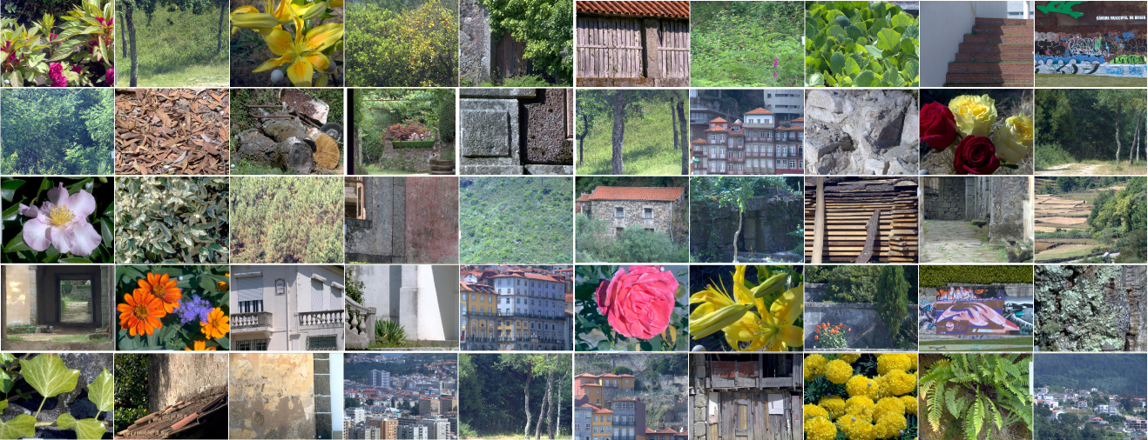
\includegraphics[width=\textwidth]{figures/foster_example.png}}{Foster}
    \caption{Objects tested under the Foster 50 Reduced Hyperspectral Reflectance Images dataset \cite{Foster2022}.}
    \label{fig:foster}
\end{figure}

\begin{figure}
    \centering
    \pdftooltip{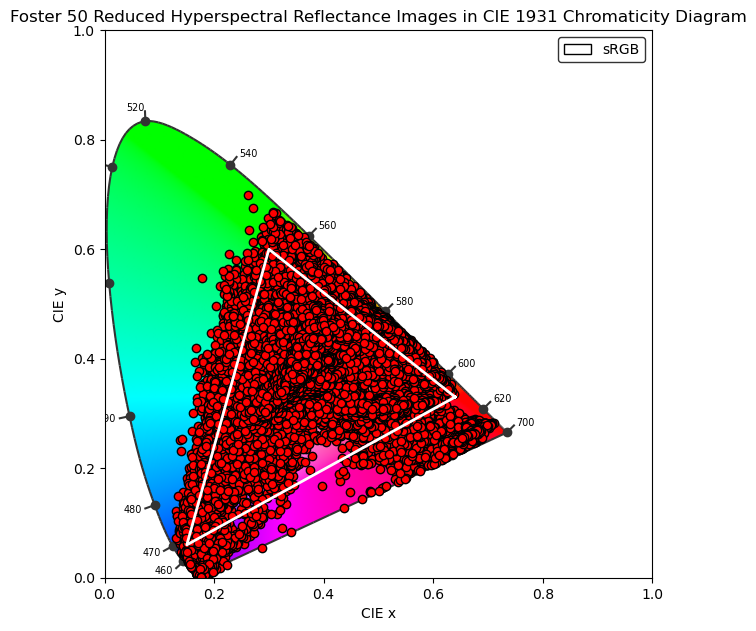
\includegraphics[scale=0.8]{figures/foster50gamut.png}}{Foster gamut}
    \caption{Chromaticity gamut of the Foster 50 Reduced Hyperspectral Reflectance Images dataset \cite{Foster2022}.}
    \label{fig:foster50gamut}
\end{figure}

Finally, we also test performance on the "In Situ Measured Spectral Radiation of Natural Objects" dataset from Image Engineering \cite{wueller2009situ}. The dataset was collected for camera colour characterisation. As such, it includes various real-life reflectance spectra, such as vegetation and human skin from different ethnicities. The dataset is packaged within the iQ-Analyzer software from Image Engineering and is publicly available for download \cite{iqanalyzer}.


\section{Camera Spectral Responses}

Since each camera has different spectral responses, the transformations from RGB to XYZ values will also vary. For example, one camera might require an aggressive transformation. In contrast, others might already have spectral sensitivities close to the human visual system, and a straightforward linear transformation might produce excellent results. In this thesis, we evaluate the results on two different cameras with very different spectral sensitivities: Nikon D5100 and Sigma SD1 Merrill. The spectral sensitivities for both cameras, published by \citeauthor{D5100NPL}, are publicly available, and the method for acquiring them is disclosed in the publication \cite{D5100NPL}.

Nikon D5100 is a standard DSLR camera with a CMOS sensor and a Bayer colour filter array. Its spectral sensitivities alongside the CIE XYZ spectra sensitivities are plotted in Figure \ref{fig:nikonvscmfs}. The figure shows that the RGB sensitivity functions (dashed) are similar to the XYZ functions (solid) in each wavelength range, indicating that a relatively simple transformation may produce good results.

\begin{figure}
    \centering
    \pdftooltip{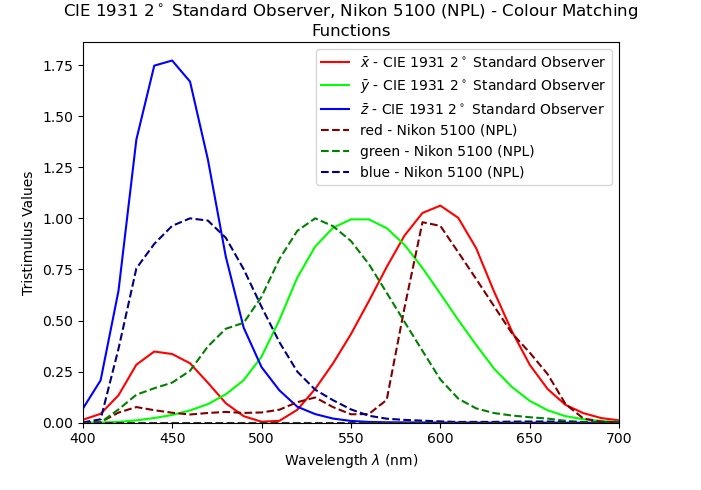
\includegraphics[width=\textwidth]{figures/nikonvscmfs.png}}{Nikon}
    \caption{Nikon D5100 \cite{D5100NPL} (dashed) vs CIE XYZ \cite{cie1931} Spectral Sensitivities (solid).}
    \label{fig:nikonvscmfs}
\end{figure}

The difference in sensor design also poses differences in the spectral sensitivities. As for the Nikon, the spectral sensitivities for Sigma SD1 Merrill are plotted in Figure \ref{fig:sigma} alongside the CIE XYZ spectral sensitivities. The different colour channels of the Sigma camera occupy a much more extensive wavelength range than the Nikon or XYZ channels do. This was also noted in \cite{finlayson2015color}, with a remark that this would lead to the Sigma requiring a more aggressive correction than, for example, the Nikon.

\begin{figure}
    \centering
    \pdftooltip{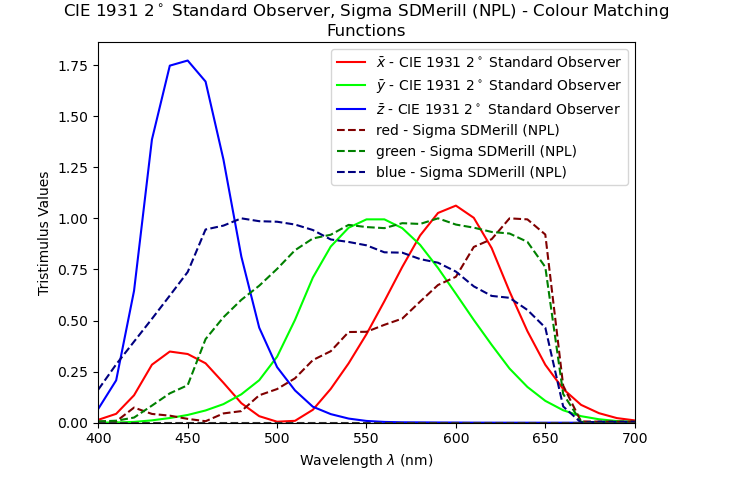
\includegraphics[width=\textwidth]{figures/sigmavscmfs.png}}{Sigma}
    \caption{Sigma SD1 Merrill \cite{D5100NPL} (dashed) vs CIE XYZ \cite{cie1931} Spectral Sensitivities (solid).}
    \label{fig:sigma}
\end{figure}



\section{Evaluation}

A software test bench was created to have similar programming interfaces across algorithms implemented using different libraries to evaluate the various algorithms presented in chapters \ref{ch:cc} and \ref{ch:proposal}. Two distinct aspects of each algorithm were tested: colour correction accuracy and robustness to changes in exposure. In both cases, we measure the performance using the CIE Delta E 2000 colour difference function in the CIELAB colour space against the responses produced by CIE 1931 Standard Observer functions.

In the subsequent analyses, models starting with "P-spline", referring to the P-spline model presented in chapter \ref{ch:proposal}, are followed by the numbers 5, 10 and 20, indicating the number of spline functions in the basis. The numbers accompanying LCC, PCC, and RPCC denote the polynomial order employed. Models suffixed with "LAB" (e.g., LCC-LAB) were optimised using the CIEDE2000 objective function within the CIELAB colour space, as per \cite{ciede2000math}. Since it does not have a closed-form solution, the Broyden–Fletcher–Goldfarb–Shanno (BFGS) algorithm, referenced in \cite{fletcher2000practical}, was employed to find the optimal solution. The network structure from \cite{macdonald2021camera} with 79 and 36 hidden layers was used for the neural network.

The neural network's learning rate and the P-spline models' penalty were found by a 5-fold cross validation (CV) before training. The dataset used for CV, in this case, the CAVE/Foster020202 dataset, was first split into five equal-sized subsets, "folds". Then, iteratively, the algorithm uses each fold once as a testing set, while the remaining datasets are used to train the model. This continues until each fold has been used as a test set once, after which we take the average of all test scores. This entire process is repeated for each hyperparameter under consideration, and in the end, each feasible hyperparameter combination has an average test score over a 5-fold CV. The model with the best score, or in this case, the lowest CIEDE2000 error, is selected as the model for training on the entire dataset and evaluated against other algorithms.

\subsection{Colour Correction Accuracy Evaluation}
 \label{ss:evaluation}

 We present our results for the Nikon D5100 in Table \ref{tab:nikon}.  When looking at models trained using the InSitu dataset, the PCC-LAB-3 model clearly produces the best mean, median and 95th percentile colour errors. In the second place, we see the P-spline-20 model, which has the lowest maximum error among all tested models and is close to the PCC-3-LAB model regarding the other metrics. The remaining models, such as the RPCC-LAB-3, tend to produce relatively higher maximum and 95th percentile errors, which can indicate worse outlier performance. For example, the standard 3rd order RPCC model has a maximum error nearly double that of the P-Spline-20 model. Overall, when trained on InSitu, the added complexity of P-spline models is not justified, as the more straightforward methods either perform comparably while being exposure-invariant (LCC-LAB) or perform better (PCC-LAB-3).

Less surprisingly, when trained on the larger CAVE/Foster020202 dataset, we see an apparent change in the rank order of the results. The simpler models, such as PCC, perform slightly worse than the P-Spline and NN models. As expected, the latter shows significant performance improvement when the amount of data is increased and takes first place in all but the maximum error metric, where it performs comparably with the simpler P-spline models. The difference in the performance of the neural network and spline model for the larger dataset is also exciting but expected. With the P-spline model, we are making assumptions on what the basis might look like for a typical camera. In contrast, with enough data, the neural networks perform this kind of analysis during training. The downside is that NNs are less interpretable due to their black-box nature.

These results also explain the difference in models' relative performance in \cite{macdonald2021camera} and \cite{kucuk2023performance}, where similar experiments were performed on Nikon D5100. In the former, the authors observed that the neural network performed better than the LCC model, while the opposite was observed in the latter experiments. The difference in the two studies, as in our experiments, was the number of training samples. In the former, the authors trained the models on datasets with 1 million samples, while in the latter, they attempted training with the number of samples ranging from only 352 to 4331. Our findings support the hypothesis that neural networks should be trained on a much larger dataset than was presented in \cite{kucuk2023performance} to see significant improvement.


 \begin{table}[htbp]
  \centering
  \caption{CIE Delta E 2000 Errors for Nikon D5100 evaluated on 50 Reduced Hyperspectral Reflectance Images (n=204800)}
    \begin{tabular}{>{\bfseries}l@{\hspace{3mm}}cccc|cccc}
        \midrule
            & \multicolumn{4}{c}{\textbf{InSitu (n=1961)}} & \multicolumn{4}{c}{\textbf{CAVE/Foster020202 (n=39935)}} \\
        \cmidrule(lr){2-5} \cmidrule(lr){6-9}
            \textbf{Algorithm} & \textbf{Mean} & \textbf{Max}  & \textbf{Median} & \textbf{P95} & \textbf{Mean} & \textbf{Max}  & \textbf{Median} &  \textbf{P95} \\
        \midrule
            P-Spline-5 & 0.76 & 5.95 & 0.67 & 1.71 & 0.94 & \textbf{4.81}  & 0.81 & 2.08 \\
            P-Spline-10 & 0.73 & 5.52 & 0.60 & 1.81 & 0.86 & 5.16 & 0.73 & 1.94 \\
            P-Spline-20 & 0.71 & \textbf{5.38} &  0.59 & 1.77 & 0.83 & 5.77 & 0.71 & 1.92 \\
            LCC & 1.01 & 8.36 & 0.89 &  2.29 & 1.00 & 5.56 & 0.86 & 2.18 \\
            LCC-LAB & 0.84 & 9.16 & 0.69 &  2.19 & 0.94 & 5.51 & 0.81 & 2.04 \\
            PCC-2 & 1.03 & 5.85 & 0.95 & 2.21 & 1.13 & 5.58 & 0.98 & 2.43 \\
            PCC-3 & 0.85 & 5.63 & 0.76 & 1.93 & 1.07 & 5.40 & 0.90 &  2.37 \\
            PCC-LAB-3 & \textbf{0.66} & 5.66 & \textbf{0.52} &  \textbf{1.70} & 0.91 & 7.07 & 0.77 &  2.03 \\
            RPCC-2 & 0.93 & 5.87 & 0.86 & 1.99 & 1.05 & 5.54 & 0.84 & 2.44 \\
            RPCC-3 & 1.02 & 9.90 &  0.91 & 2.32 & 1.06 & 5.69 & 0.85 & 2.43 \\
            RPCC-LAB-3 & 0.72 & 7.33 & 0.58 & 1.83 & 0.92 & 8.04 & 0.76 & 2.22 \\
            NN & 16.11 & 50.91 & 15.73 & 28.01 & \textbf{0.67} & 4.87 & \textbf{0.54} & \textbf{1.66} \\
        \bottomrule
    \end{tabular}
  \label{tab:nikon}
\end{table}

In Table \ref{tab:sigma} are the results for Sigma SD Merrill, also trained using the InSitu dataset and combination of CAVE and Foster02 (CAVE/Foster02) datasets, and finally tested on the Foster 50 Reduced Hyperspectral Reflectance Images (Foster50) dataset. At first glance, it is clear that the transformation from RGB to XYZ is significantly more challenging for Sigma than for Nikon, as the mean and maximum errors are three to four times as high. This supports the observation of \citeauthor{finlayson2015color} that the transformation for the camera is more complex due to the breadth of each channel's spectral sensitivities.

Unlike the results for Nikon in table \ref{tab:nikon}, we see that most algorithms perform similarly when trained on the larger CAVE/Foster02 dataset compared to the InSitu dataset. The proposed P-spline models also consistently outperform the other polynomial models, even in the simple case when using just five basis functions, which can be attributed to the ability to take local variations in the transformation into account. 

Similarly to Nikon, the NNs perform much worse when the training dataset is smaller but see a significant improvement as we increase the size. A similar hypothesis is plausible for this as was for Nikon; although splines are flexible as basis functions, NNs can form a more accurate transform based on the data distributions. Furthermore, since the Sigma sensitivities are much different compared to the HVS, the smoothness of our P-spline model may not be able to form a sufficiently aggressive transform.

\begin{table}[htbp]
  \centering
  \caption{CIE Delta E 2000 Errors for Sigma SD Merrill evaluated on 50 Reduced Hyperspectral Reflectance Images (n=204800)}
    \begin{tabular}{>{\bfseries}l@{\hspace{3mm}}cccc|cccc}
        \midrule
            & \multicolumn{4}{c}{\textbf{InSitu (n=1961)}} & \multicolumn{4}{c}{\textbf{CAVE/Foster0202 (n=39935)}} \\
        \cmidrule(lr){2-5} \cmidrule(lr){6-9}
            \textbf{Algorithm} & \textbf{Mean} & \textbf{Max} & \textbf{Median} & \textbf{P95} & \textbf{Mean} & \textbf{Max} & \textbf{Median} & \textbf{P95} \\
        \midrule
            P-Spline-5 & \textbf{1.88} & 22.92 & \textbf{1.24} & 6.06 & 1.77 & 18.27 & 1.45 & 4.14 \\
            P-Spline-10 & 1.99 & 22.87 & 1.35 & 6.23 & 1.74 & 17.74 & 1.44 & 4.03 \\
            P-Spline-20 & 1.94 & \textbf{21.99} & 1.33 & 5.99 & 1.73 & 16.95 & 1.46 & 4.00 \\
            LCC & 2.27 & 23.25 & 1.67 & 6.72 & 2.20 & 23.49 & 1.52 & 6.98 \\
            LCC-LAB & 2.28 & 22.56 & 1.78 & 6.32 & 2.57 & 19.60 & 2.15 & 5.59 \\
            PCC-2 & 2.16 & 22.75 & 1.57 & 6.31 & 2.02 & 22.07 & 1.49 & 5.82 \\
            PCC-3 & 1.91 & 22.50 & 1.30 & 6.04 & 1.92 & 20.78 & 1.49 & 5.01 \\
            PCC-3-LAB & 1.96 & 22.43 & 1.33 & 6.23 & 1.98 & 17.92 & 1.74 & 4.42 \\
            RPCC-2 & 2.08 & 26.03 & 1.42 & 6.45 & 2.17 & 25.38 & 1.50 & 6.84 \\
            RPCC-3 & 2.27 & 42.86 & 1.49 & 6.38 & 2.32 & 34.32 & 1.65 & 6.90 \\
            RPCC-3-LAB & 1.93 & 31.63 & 1.30 & \textbf{5.89} & 2.02 & 43.46 & 1.36 & 5.54 \\
            NN & 17.77 & 56.10 & 17.58 & 29.21 & \textbf{1.55} & \textbf{16.17} & \textbf{1.24} & \textbf{3.89} \\
        \bottomrule
    \end{tabular}
  \label{tab:sigma}
\end{table}

\subsection{Spline Transformation Analysis}

In addition to finding a more flexible model, this thesis aimed to understand the nature of the transformations behind colour correction. Thanks to their flexibility, more complex models, such as P-splines with large bases, can adapt to various functions while still being robust in practice due to the incorporated smoothing factor. Since they follow the classical regression models, it is possible to observe and visualise the effect of individual features on the final output while nullifying the impact of other input features. This is called partial dependence and can be used to interpret regression models.

With P-spline models using two-way tensor product splines, it is possible to form a three-dimensional visualisation where we observe the partial dependence of each tensor product separately. Since our input features, in terms of tensor products, consist of $(\mathbf{r} \otimes \mathbf{g}, \mathbf{r} \otimes \mathbf{b}, \mathbf{g} \otimes \mathbf{g})$, in each plot we consider one tensor product's effect on one of the output variables ($X$, $Y$ or $Z$).


Figure \ref{fig:nikonspline} shows the partial dependencies for each tensor product term in predicting the Y-component for the Nikon camera P-spline models with 5, 10, and 20 basis functions, respectively. The red points among the surfaces indicate the location of control points for each term. From these, we can observe that the transformations at first appear similar, suggesting they are attempting to model a comparable underlying surface. However, the increased number of basis functions allows us to adapt to variations in the transformation, and as such, we observe slight differences in curvature between models. Of course, the curvature depends on the number of basis functions and the penalisation parameter $\lambda$, found through hyperparameter optimisation on the training dataset for each P-spline model separately. 

\begin{figure}
    \centering
    \pdftooltip{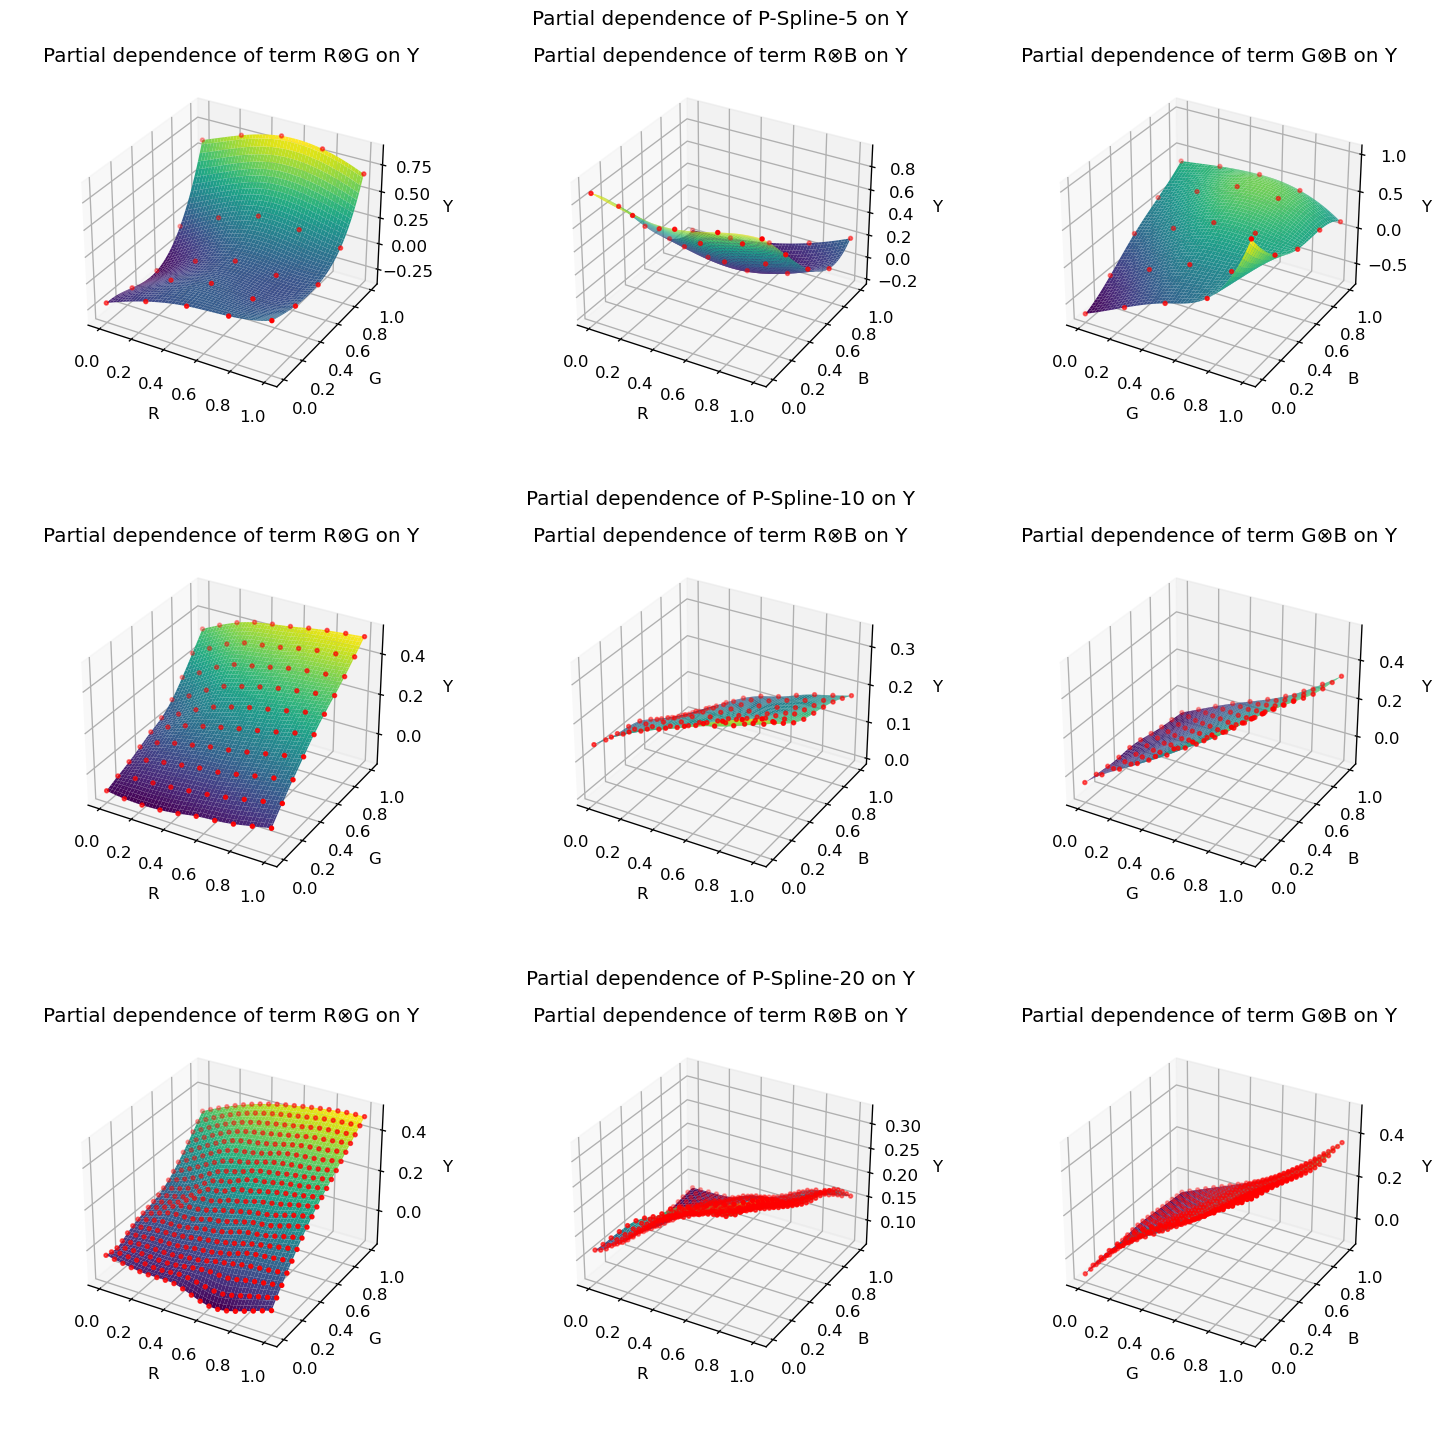
\includegraphics[width=\textwidth]{figures/nikon_pspline_20.png}}{Spline Fit, Nikon}
    \caption{Nikon D5100 partial dependencies of different terms on the predicted Y-component for P-spline models with 5, 10 and 20 basis functions.}
    \label{fig:nikonspline}
\end{figure}

Figure \ref{fig:sigmaspline} shows a plot showcasing the same setup for the Sigma SD Merrill. By comparing these figures to their counterparts for Nikon D5100 in figure \ref{fig:nikonspline}, it is clear that the underlying transformation is different for the two cameras, with the Sigma requiring more aggressive correction. In line with our results, we saw minimal curvature in fitted surfaces for the Nikon and observed that the simpler polynomial models produce better results. In contrast, we observed better results for the Sigma with the more flexible and complex P-spline models.

\begin{figure}
    \centering
    \pdftooltip{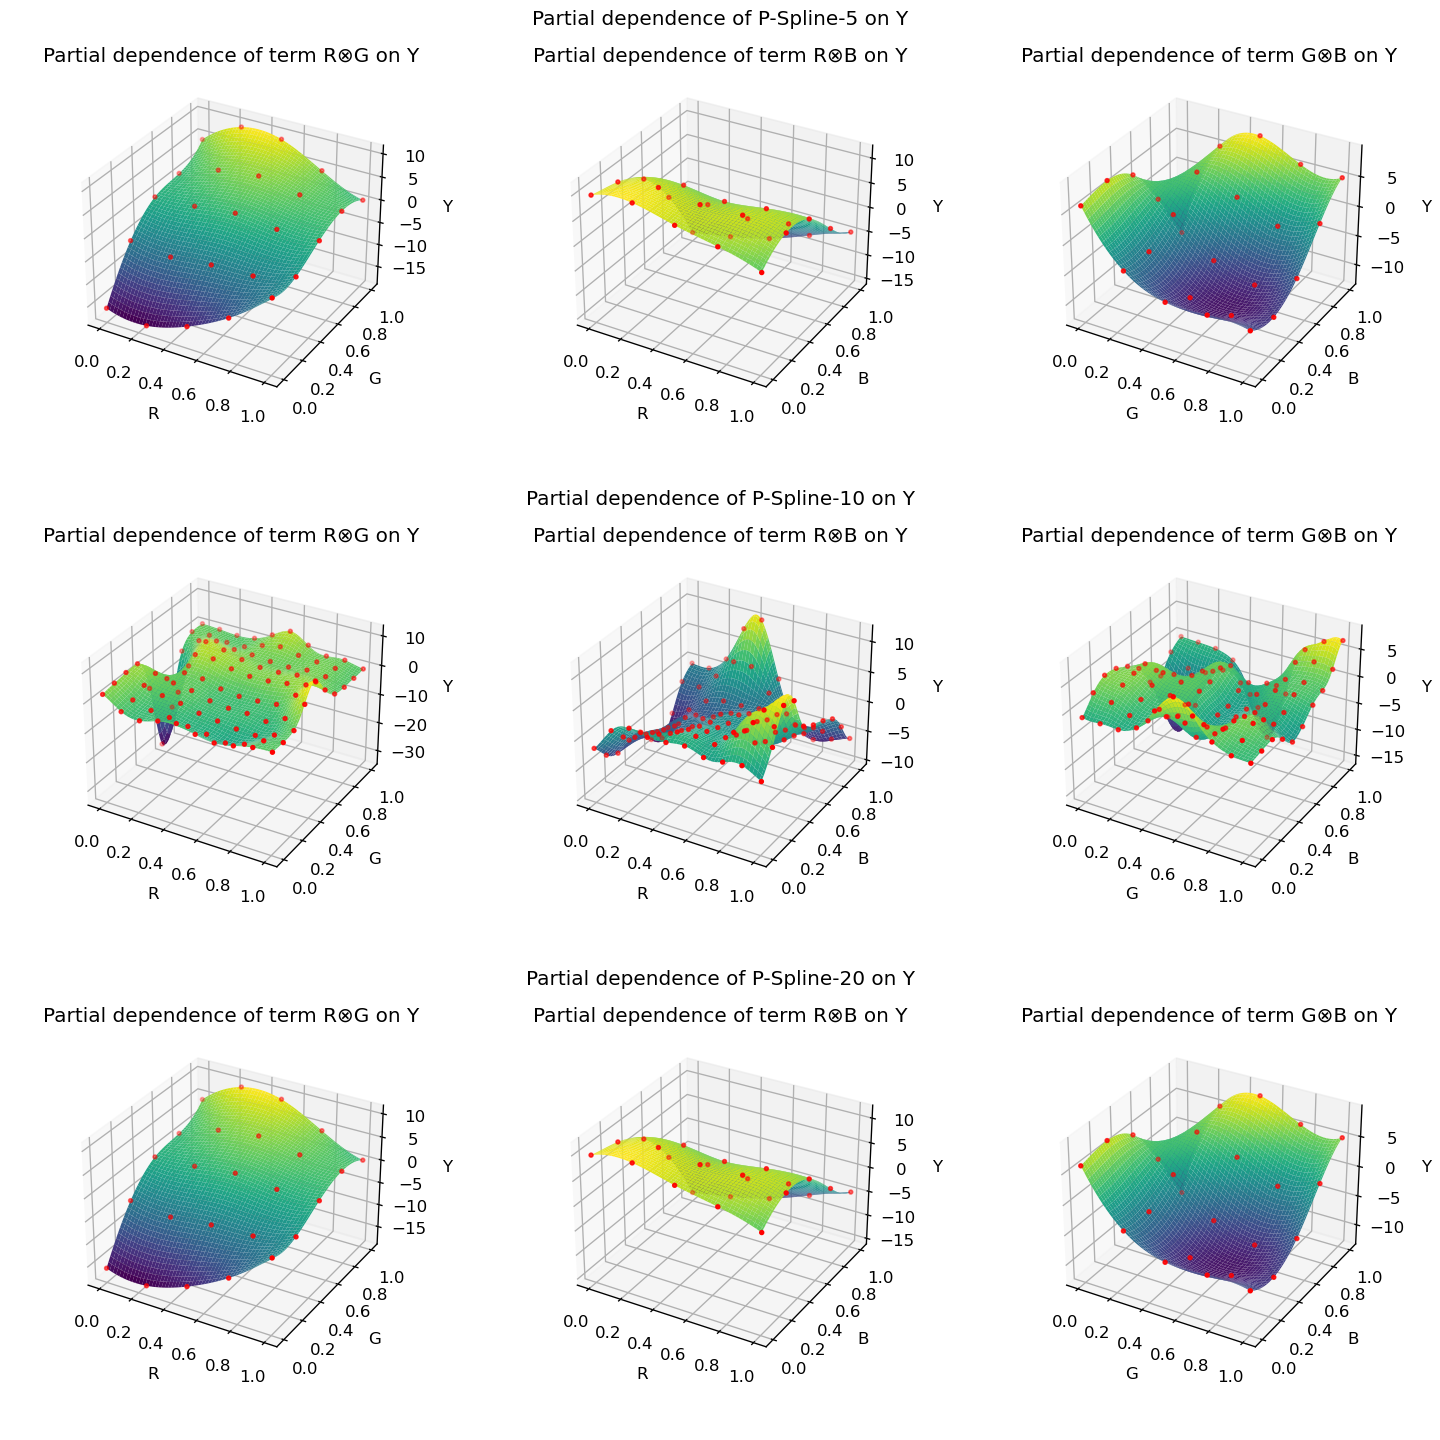
\includegraphics[width=\textwidth]{figures/sigma_pspline_20.png}}{Spline Fit, Sigma}
    \caption{Sigma SD Merrill partial dependencies of different terms on the predicted Y-component for P-spline models with 5, 10 and 20 basis functions.}
    \label{fig:sigmaspline}
\end{figure}

Yet another way to interpret the resulting transformations is to observe how good of a fit can be found directly in the spectral domain. Theoretically, the only cause of discrepancies in the responses formed by an image sensor and HVS is their spectral sensitivities, as they sample the incoming light differently wavelength-per-wavelength.

Figures \ref{fig:nikonfit} and \ref{fig:sigmafit} show the P-spline spectral fit to the CIE 1931 CMFs for Nikon and Sigma with 5, 10 and 20 basis functions, respectively. By visual observation, in both cases, they all seem to produce close to an exact fit in the spectral domain. Contrary to the results in Tables \ref{tab:nikon} and \ref{tab:sigma}, where Sigma had higher errors for all presented P-spline models, we observe the opposite results in the spectral domain.

Two things can explain the difference in performance across domains. Firstly, since the errors are not evenly distributed across the wavelength range, the amount of error accumulated in the XYZ domain is amplified by the incident stimulus, such as daylight. Second, we are working in the response rather than the spectral domain in practical spectral calibration. The goodness of a fit is then also affected by the number and quality of training samples. Two different stimuli can also produce the same response for a human eye but not an image sensor, resulting in a phenomenon called observer metamerism, which was discussed in \ref{ss:metamerism}.

\begin{figure}
    \centering
    \pdftooltip{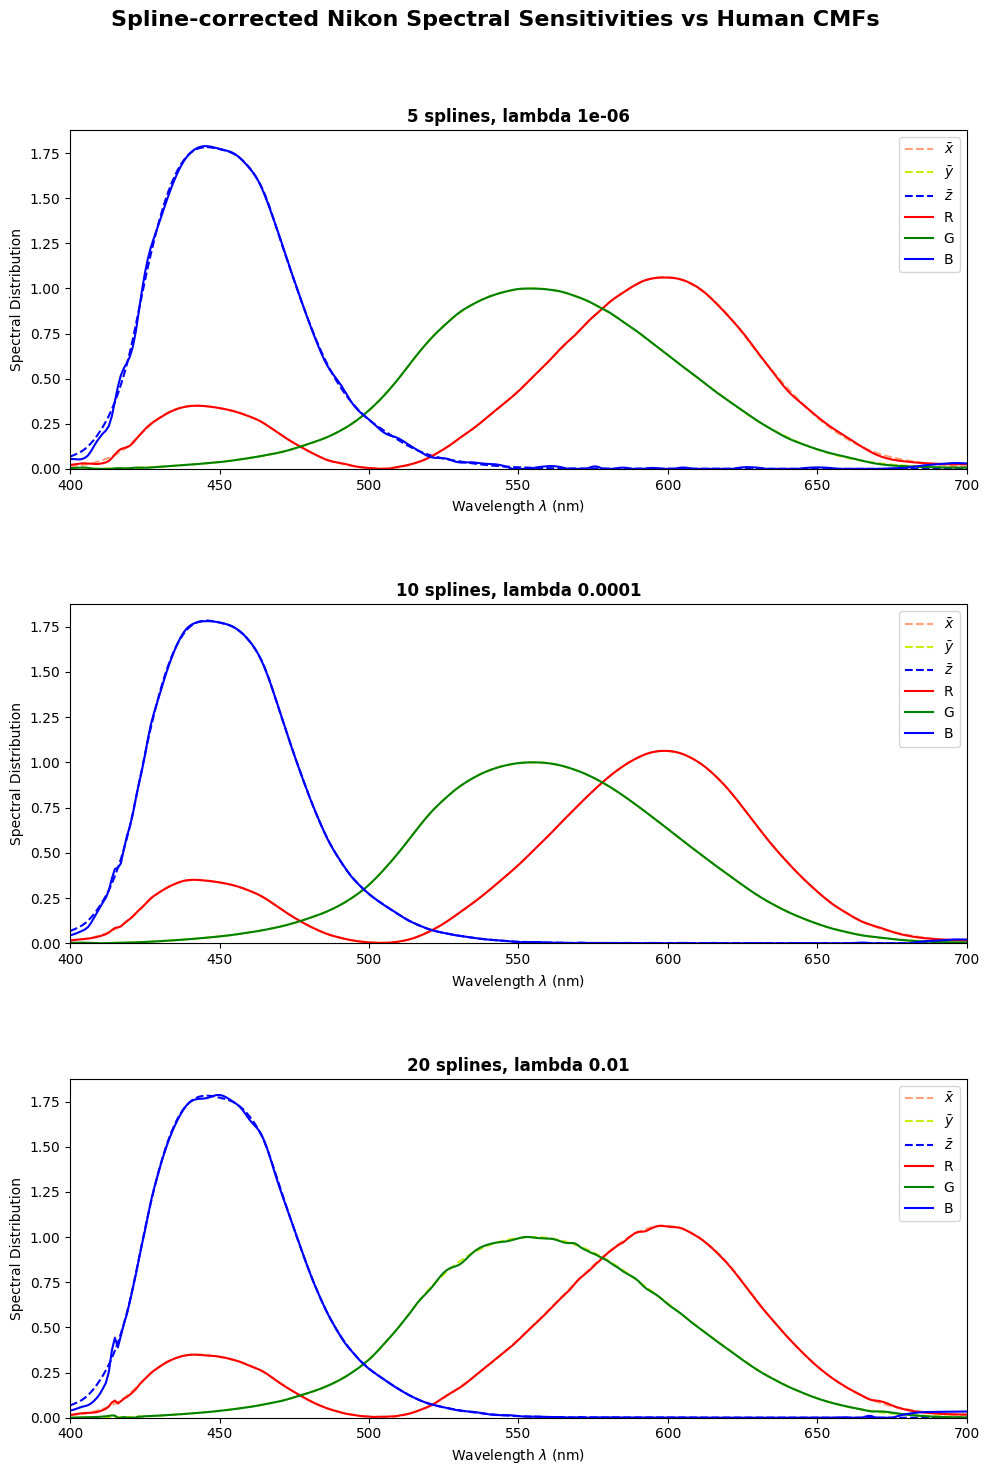
\includegraphics[width=\textwidth]{figures/nikonfit.png}}{Spectral fit, Nikon}
    \caption{Nikon D5100 SSF fit to the 1931 CMFs for P-spline models with 5, 10 and 20 basis functions.}
    \label{fig:nikonfit}
\end{figure}


\begin{figure}
    \centering
    \pdftooltip{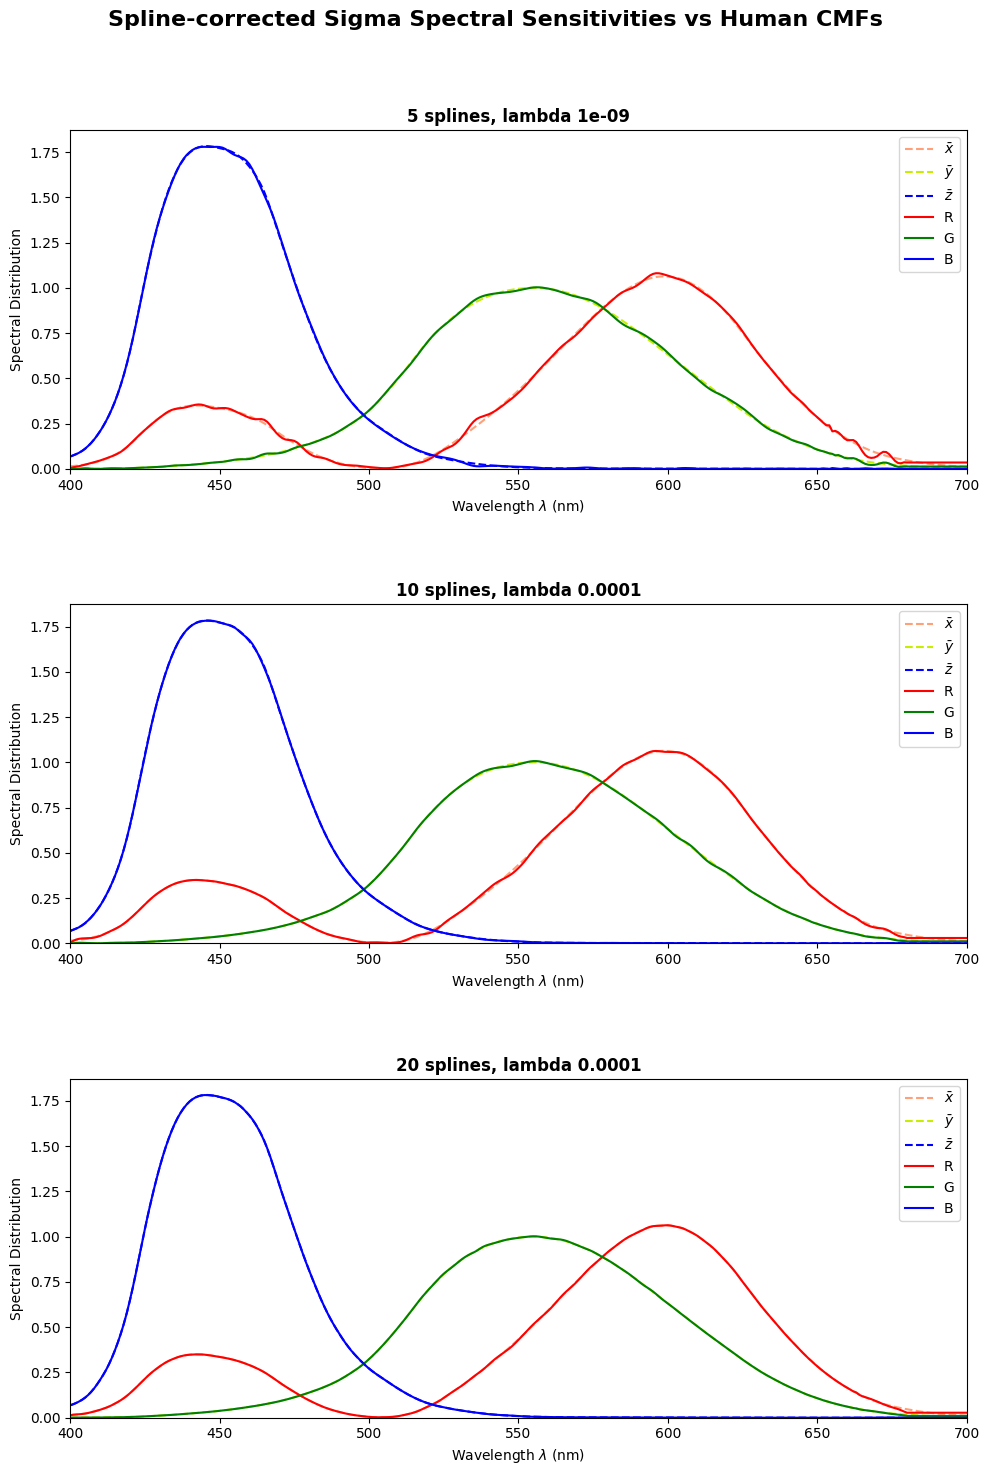
\includegraphics[width=\textwidth]{figures/sigmafit.png}}{Spectral fit, Sigma}
    \caption{Sigma SD Merrill SSF fit to the 1931 CMFs for P-spline models with 5, 10 and 20 basis functions.}
    \label{fig:sigmafit}
\end{figure}

\subsection{Exposure Invariance}

Exposure invariance and colour correction accuracy are among the most essential properties of a colour correction algorithm. For some algorithms, such as the LCC and RPCC, this is an inherent feature of the algorithms due to the mathematical properties discussed in chapter \ref{ch:cc}. Other models, such as PCC or neural networks, do not have this property by nature, although the former can be trained to be robust across exposures by data augmentation or design \cite{kucuk2022exposure}.

To our knowledge, no experiments regarding performance across different exposures have been conducted for spline-based models. While splines can suffer from problems similar to PCC in being highly non-linear and thus exposure-invariant, in some regions, it can also be controlled by tuning the amount of penalisation $\lambda$, with higher values leading the model increasingly towards a linear model. Here, we explore whether we can make the models exposure-invariant by controlling $\lambda$.

We perform our experiments as follows: Instead of using training and test sets from separate distributions, we perform a 5-fold cross-validation on the InSitu dataset, similar to in previous exposure invariance tests from the literature \cite{kucuk2022exposure}, \cite{finlayson2015color}.
Since the exposure invariance of the other models evaluated in section \ref{ss:evaluation} has already been explored in the literature, interested readers may refer to \cite{finlayson2015color}, \cite{kucuk2022comparison}, \cite{kucuk2022exposure} and \cite{kucuk2023performance} for more information.

To test the performance across exposure change, we multiply the input RGB values by the following scalars one at a time: $1/5$, $1/2$, $1$, and $2$. For this purpose, we consider our synthetic sensor's potential values to be between $0$ and $1$, e.g. normalising the FWC to 1. To avoid clipping, before evaluation, we remove samples that would clip when evaluated at exposure of 2. Furthermore, after predicting the target XYZ values, we scale them back to an exposure of 1 by dividing by the current exposure. This has the following advantage: for an exposure invariant model, such as the LCC, the errors will be the same as for the case of exposure of 1. If the model does not have the same errors along different exposure levels after division, they are not exposure-invariant.

In Figure \ref{fig:nikonexposure}, we plot the mean CIEDE2000 error for Nikon D5100 as a function of $\lambda$, ranging from \num{1e-9} to \num{5e-1}, for the exposures mentioned above when trained on the InSitu dataset. As expected, all P-spline models suffer from high errors when little penalisation is applied in the case of exposure 2. As we approach the end of the x-axis, the mean error converges to roughly the same number for all exposure levels across all spline models. We see similar results for the Sigma SD Merrill in figure \ref{fig:sigmaexposure}, where the models start to converge towards exposure-invariance at approximately \num{1e-1}, aside from the simpler P-Spline-5 model that has near-constant error starting from \num{1e-5}.

\begin{figure}
    \centering
    \pdftooltip{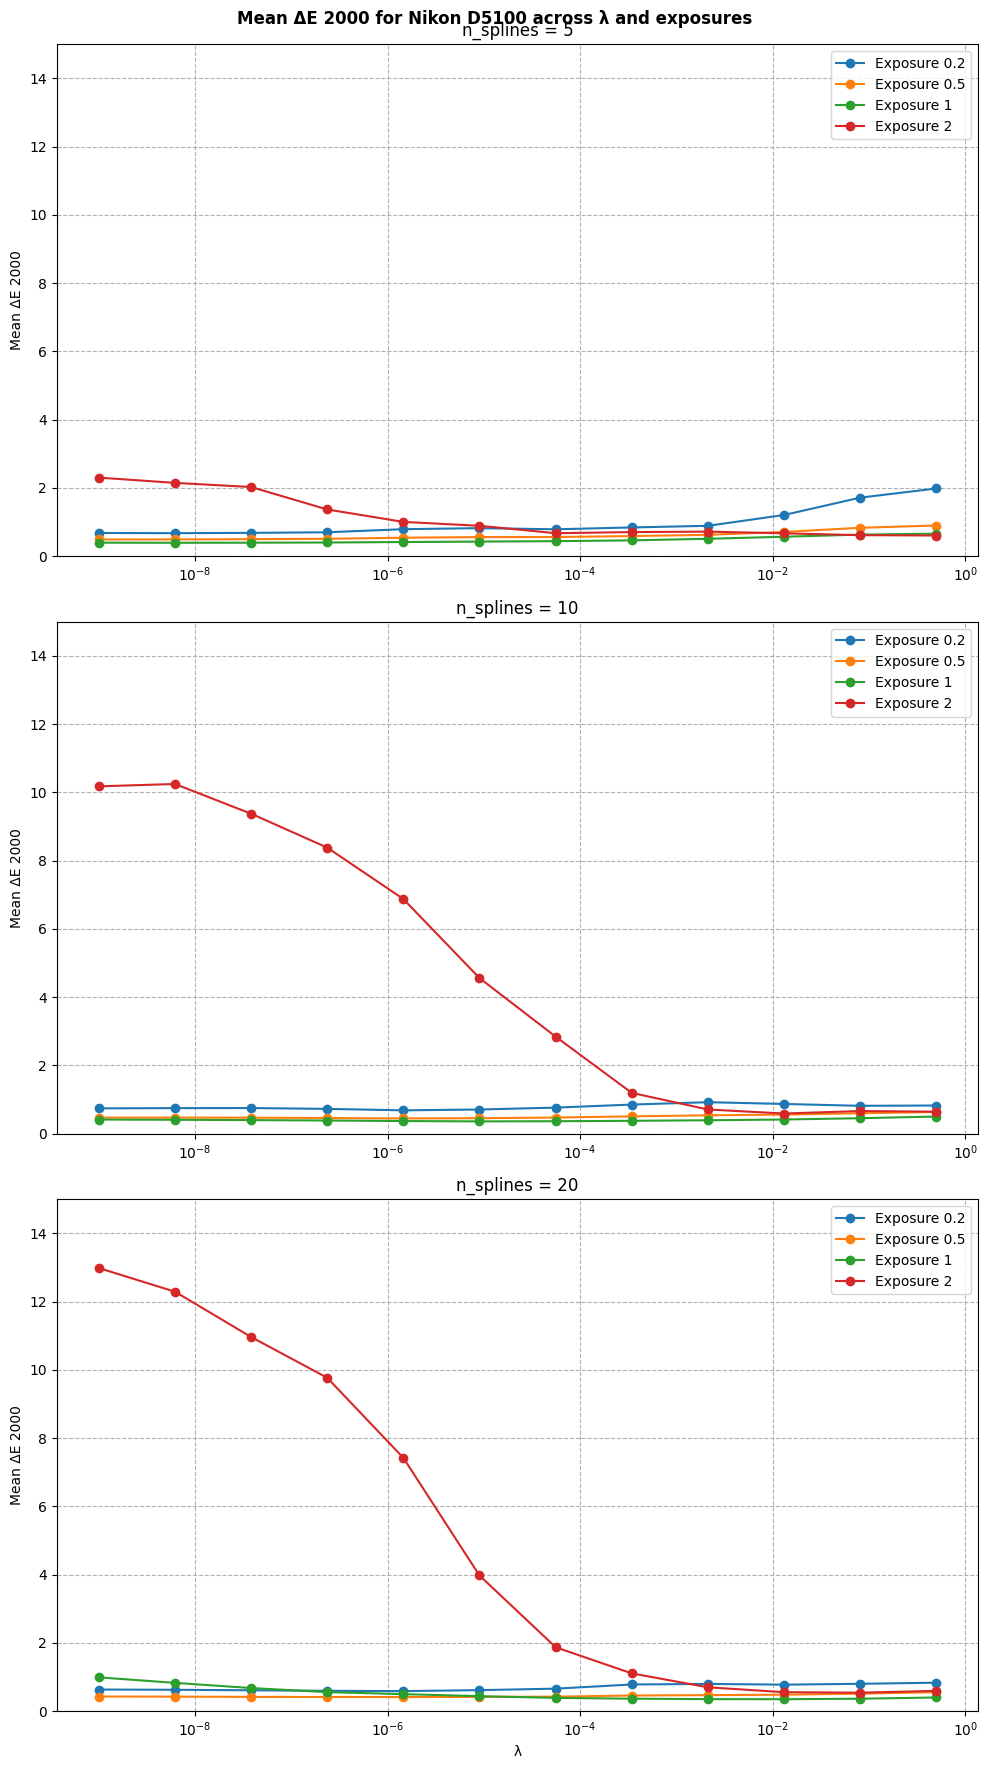
\includegraphics[width=0.85\textwidth]{figures/nikonexposure.png}}{Nikon Exposure Invariance}
    \caption{Mean CIE DeltaE 2000 for Nikon D5100 across penalties $\lambda$ and exposures.}
    \label{fig:nikonexposure}
\end{figure}

\begin{figure}
    \centering
    \pdftooltip{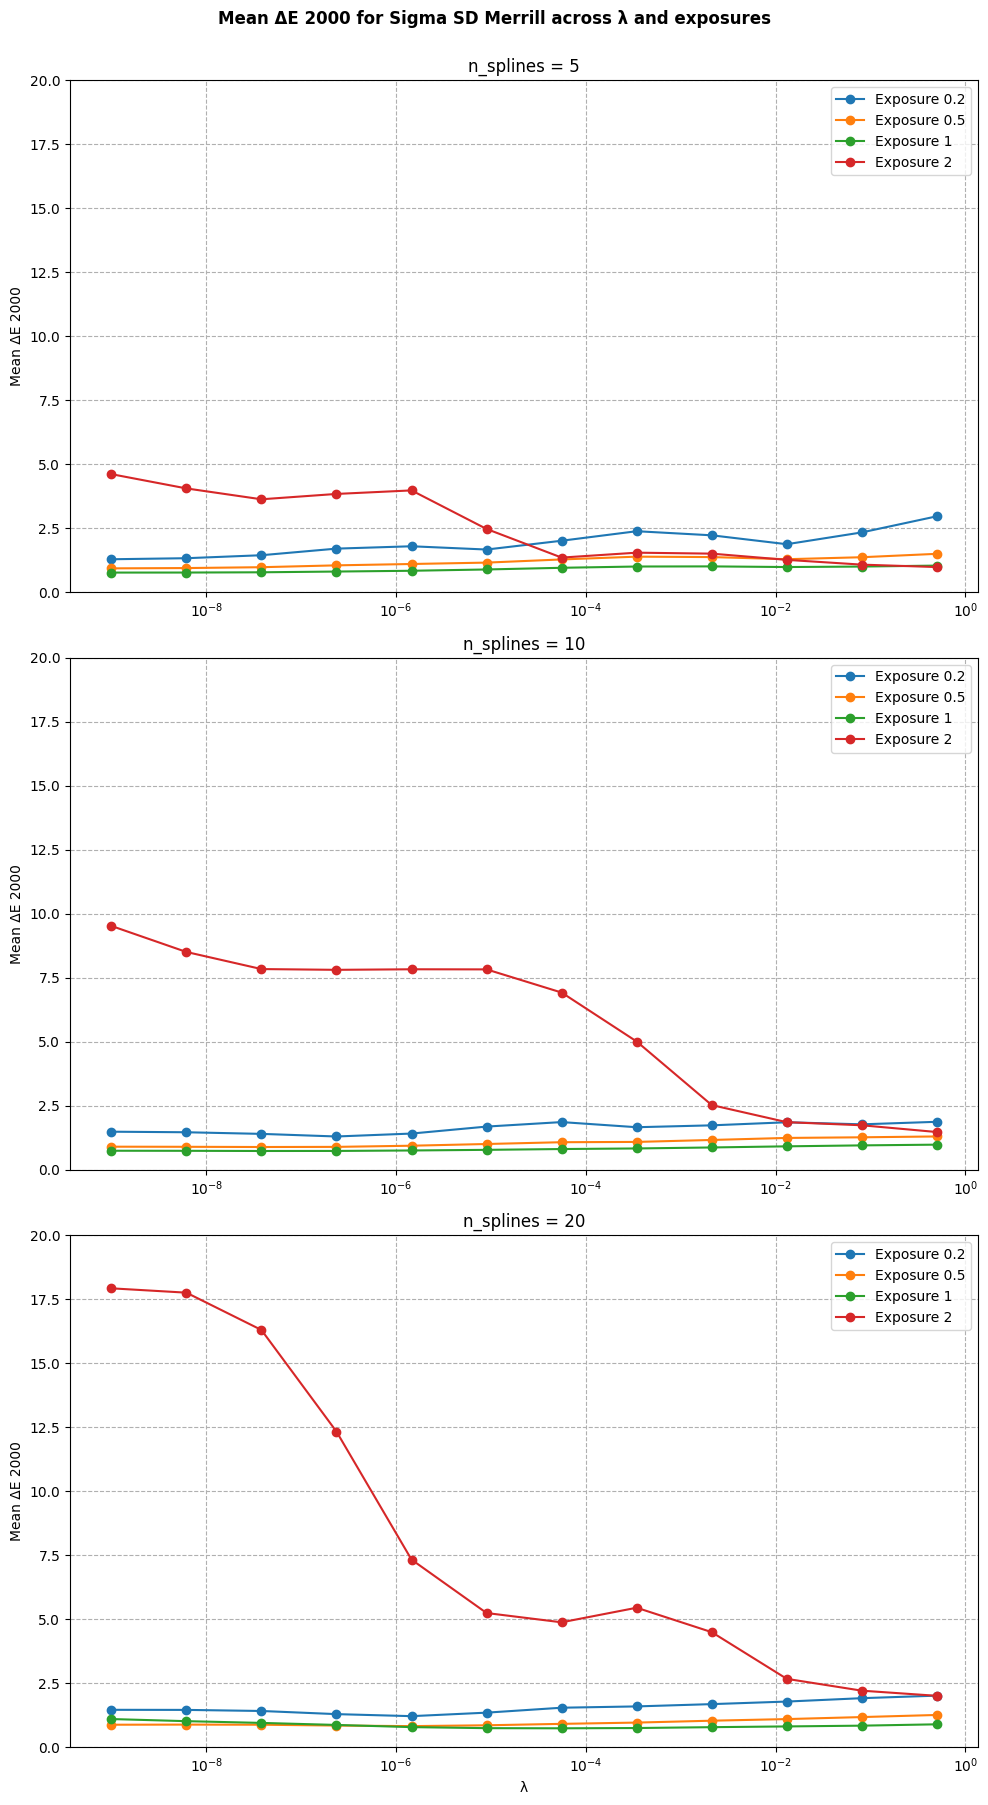
\includegraphics[width=0.85\textwidth]{figures/sigmaexposure.png}}{Sigma Exposure Invariance}
    \caption{Mean CIE DeltaE 2000 for Sigma SD Merrill across penalties $\lambda$ and exposures.}
    \label{fig:sigmaexposure}
\end{figure}

It is to be noted that while the error across exposures gets smaller for both cameras as we start to penalise the model, it does not come for free. Since the key idea of splines is to allow local rather than global variation in the transformation, the flexibility is reduced with increased penalisation factor $\lambda$. Having only a single value of $\lambda$ tuned for the entire model further restricts the variation. As such, local penalisation could achieve better results, for example, by making the neutral (achromatic) axis of the transformation linear while allowing the rest of the surface to vary. This property is also utilised in the RPCC model, for which it is a natural property, although the global nature limits the variation outside the neutral axis.